\documentclass[12pt]{article}
\usepackage[margin=1in]{geometry}
\usepackage{amsmath,amssymb,amsthm}
\usepackage{tikz}
\usepackage{graphicx}
\usepackage{enumerate}
\usepackage{hyperref}
\usetikzlibrary{trees,positioning,arrows.meta}

\title{CS5383 Theory of Automata\\
Homework 1: Course Introduction\\
Representing and Reasoning with Concepts and Statements}
\author{Scott Weeden\\
Texas Tech University}
\date{September 17, 2025}

\theoremstyle{definition}
\newtheorem{definition}{Definition}
\newtheorem{theorem}{Theorem}
\newtheorem{lemma}{Lemma}

\begin{document}
\maketitle

\section*{Introduction}
This homework explores the foundational concepts of automata theory and their profound connections to computational reasoning, pattern recognition, and abstract problem-solving. As a Data Analyst and Machine Learning specialist participating in the ARC Challenge, I find these theoretical foundations particularly relevant to understanding how machines can learn to recognize and manipulate abstract patterns—a core requirement for both automata theory and the ARC Challenge.

\section*{Question 1: Acknowledgments}
\textbf{Contributors to this solution:}
\begin{itemize}
    \item Claude AI: Assisted with LaTeX formatting, provided insights on connecting automata theory to the ARC Challenge, and helped structure mathematical definitions.
    \item Online Resources: Stanford Encyclopedia of Philosophy for formal logic structures, MIT OpenCourseWare for automata theory applications.
\end{itemize}

\section*{Question 2: Academic Integrity}
I hereby acknowledge that I have read and understood the academic integrity policy for CS5383. I commit to submitting only my own original work and properly citing all sources of assistance.

\textit{[Signature placeholder]}

\section*{Question 3: Course Materials Review}
\textbf{Response: Strongly Agree}

After completing this homework, I strongly agree with the statement about studying class materials before assignments. The concepts of formal language representation, precise mathematical definitions, and reasoning about computational limits directly mirror the challenges in the ARC dataset, where one must identify abstract patterns and apply logical transformations. The lecture materials on representing concepts as functions and statements as programs provides a crucial framework for approaching both automata problems and ARC puzzles systematically.

\section*{Question 4: Relevance of Automata Theory}
After researching the applications of automata theory, the three most relevant reasons for my interests as a Data Analyst and ARC Challenge participant are:

\subsection*{1. Pattern Recognition and Abstract Reasoning}
Automata theory provides formal frameworks for recognizing patterns in sequences—a skill directly applicable to the ARC Challenge. Finite automata model pattern recognition systems that must identify regularities in grids and sequences, similar to how ARC tasks require identifying transformation rules from limited examples. The mathematical rigor of automata helps formalize what it means to "understand" a pattern.

\subsection*{2. Computational Limits and Decidability}
Understanding the hierarchy of computational power (finite automata $\subset$ pushdown automata $\subset$ Turing machines) illuminates what problems can be solved algorithmically. This is crucial for the ARC Challenge, which tests whether AI systems can perform abstract reasoning tasks that humans find intuitive but machines struggle with. Knowing these limits helps identify which approaches might succeed or fail.

\subsection*{3. Formal Language Processing for Machine Learning}
Regular expressions and context-free grammars, core topics in automata theory, underpin many ML preprocessing pipelines. In data analysis, we constantly parse structured data, validate inputs, and transform sequences. The formal methods from automata theory ensure correctness and efficiency in these operations, while also providing insights into feature engineering for sequence-based learning tasks.

\section*{Question 5: Concepts as Functions, Statements as Programs}
\textbf{Yes, I have frequently linked these abstractions, and your connection makes perfect sense.}

In machine learning, we constantly treat concepts as functions:
\begin{itemize}
    \item A classifier is literally a function $f: X \rightarrow Y$ mapping inputs to concepts
    \item Feature extractors are functions that compute properties of data
    \item Neural network layers are compositions of functions
\end{itemize}

Statements as programs is equally natural:
\begin{itemize}
    \item SQL queries are statements that compile to execution plans
    \item Declarative ML frameworks (like TensorFlow's graph mode) specify what to compute rather than how
    \item The ARC Challenge itself presents visual "statements" that must be interpreted as transformation programs
\end{itemize}

This connection crystallizes how theoretical computer science provides the mathematical foundation for practical AI systems.

\section*{Question 6: Components and Use of Concepts}
\subsection*{Components of a Concept:}
A concept consists of:
\begin{enumerate}
    \item \textbf{Name/Identifier}: A label that references the concept (e.g., "parent", "regular language")
    \item \textbf{Parameters/Arguments}: Variables that the concept operates on (e.g., X and Y in "X is parent of Y")
    \item \textbf{Definition/Body}: The precise conditions or rules that determine when the concept applies
    \item \textbf{Domain}: The set of valid inputs for the parameters
\end{enumerate}

\subsection*{Use of a Concept:}
The "use of a concept" means instantiating it with specific arguments to create a statement or proposition. For example, using the concept "parent(X,Y)" with arguments "Sarah" and "Ryan" creates the statement "parent(Sarah, Ryan)".

\subsection*{Precise/Mathematical Definition:}
A definition is precise or mathematical when:
\begin{itemize}
    \item It uses unambiguous formal language
    \item All terms are either primitive or previously defined
    \item The conditions for truth are deterministic and verifiable
    \item It avoids natural language ambiguities
\end{itemize}

\section*{Question 7: Pumping Lemma Analysis}

\subsection*{(a) Concept Identification}

\textbf{Known Concepts:}
\begin{itemize}
    \item exists ($\exists$): existential quantifier
    \item for all ($\forall$): universal quantifier
    \item such that: logical connector
    \item $\geq$, $\leq$: inequality relations
    \item decomposed: partitioning operation
    \item depends on: functional dependency
\end{itemize}

\textbf{New Concepts (Domain-Specific):}
\begin{itemize}
    \item regular language (L): a formal language recognizable by finite automata
    \item alphabet ($\Sigma$): finite set of symbols
    \item $w \in L$: string membership in language
    \item $|w|$: string length function
    \item $\epsilon$: empty string
    \item $xy^kz$: string concatenation with repetition
    \item constant n: pumping length
\end{itemize}

\subsection*{(b) Tree Structure of Pumping Lemma}

\begin{center}
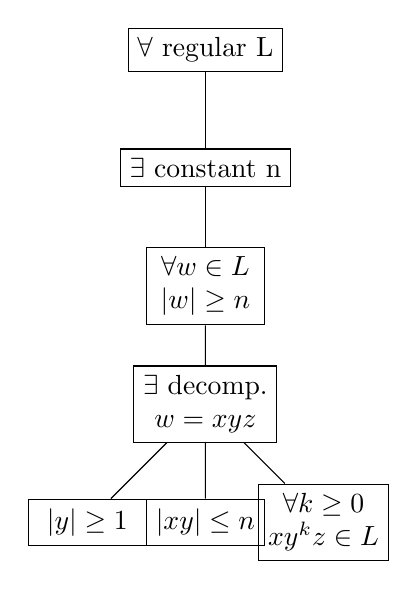
\begin{tikzpicture}[
    level distance=1.5cm,
    level 1/.style={sibling distance=6cm},
    level 2/.style={sibling distance=3cm},
    level 3/.style={sibling distance=1.5cm},
    every node/.style={draw, rectangle, align=center, minimum width=1.5cm},
    arrow/.style={->, thick}
]
\node {$\forall$ regular L}
    child {node {$\exists$ constant n}
        child {node {$\forall w \in L$\\$|w| \geq n$}
            child {node {$\exists$ decomp.\\$w = xyz$}
                child {node {$|y| \geq 1$}}
                child {node {$|xy| \leq n$}}
                child {node {$\forall k \geq 0$\\$xy^kz \in L$}}
            }
        }
    };
\end{tikzpicture}
\end{center}

\section*{Question 8: Parent Statement Analysis}

\subsection*{1) Use of Concepts:}
\begin{itemize}
    \item Concept: \texttt{parent(X, Y)}
    \item Arguments: \texttt{X = Sarah, Y = Ryan}
    \item Statement: \texttt{parent(Sarah, Ryan)}
\end{itemize}

\subsection*{2) Application of L2 Definition:}
Applying the definition from L2:
\begin{align}
\text{parent(Sarah, Ryan)} &\equiv \text{father(Sarah, Ryan)} \vee \text{mother(Sarah, Ryan)}
\end{align}

Tree structure:
\begin{center}
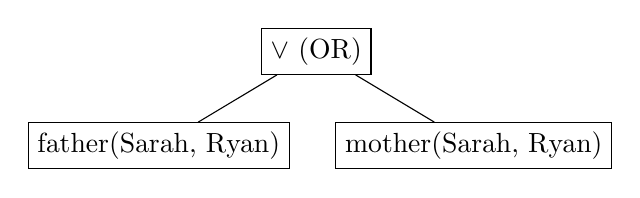
\begin{tikzpicture}[
    level distance=1.2cm,
    level 1/.style={sibling distance=4cm},
    every node/.style={draw, rectangle, align=center},
]
\node {$\vee$ (OR)}
    child {node {father(Sarah, Ryan)}}
    child {node {mother(Sarah, Ryan)}};
\end{tikzpicture}
\end{center}

\subsection*{3) Truth Value:}
Given biological constraints where "Sarah" is typically a female name:
\begin{itemize}
    \item \texttt{father(Sarah, Ryan) = FALSE} (Sarah cannot be a father)
    \item \texttt{mother(Sarah, Ryan) = TRUE} (Sarah can be a mother)
    \item Therefore: \texttt{parent(Sarah, Ryan) = TRUE}
\end{itemize}

\section*{Question 9: Proof that Sarah is a Parent of Ryan}

\begin{proof}[Working Backwards Proof]
\textbf{Goal:} Prove that \texttt{parent(Sarah, Ryan)} is true.

\textbf{Step 1:} By definition of parent in L2:
\[\text{parent(Sarah, Ryan)} \equiv \text{father(Sarah, Ryan)} \vee \text{mother(Sarah, Ryan)}\]

\textbf{Step 2:} To prove a disjunction, we need to prove at least one disjunct is true.

\textbf{Step 3:} We claim \texttt{mother(Sarah, Ryan)} is true.

\textbf{Step 4:} By the definition of mother:
\[\text{mother(Sarah, Ryan)} \equiv \text{female(Sarah)} \wedge \text{biological\_parent(Sarah, Ryan)}\]

\textbf{Step 5:} We establish:
\begin{itemize}
    \item \texttt{female(Sarah) = TRUE} (given: Sarah is a female name)
    \item \texttt{biological\_parent(Sarah, Ryan) = TRUE} (given: biological relationship exists)
\end{itemize}

\textbf{Step 6:} Since both conjuncts are true:
\[\text{mother(Sarah, Ryan)} = \text{TRUE}\]

\textbf{Step 7:} Since \texttt{mother(Sarah, Ryan)} is true and it's one disjunct of the parent definition:
\[\text{parent(Sarah, Ryan)} = \text{TRUE}\]

Therefore, Sarah is a parent of Ryan. \qed
\end{proof}

\section*{Question 10: Precise Definitions}

\subsection*{(a) Definition of Grandparent}
\begin{definition}[Grandparent]
Let $X$ and $Y$ be individuals. We say "$X$ is a grandparent of $Y$" if and only if:
\[\exists Z \: [\text{parent}(X, Z) \wedge \text{parent}(Z, Y)]\]

In expanded form:
\[\text{grandparent}(X, Y) \equiv \exists Z \: [\text{parent}(X, Z) \wedge \text{parent}(Z, Y)]\]

where $Z$ ranges over all individuals in the domain.
\end{definition}

\subsection*{(b) Identity Matrix Definition}

\subsubsection*{i. Critique of Original Definition}
The definition in Figure 1 suffers from:
\begin{enumerate}
    \item \textbf{Ambiguous notation}: Uses "$1$" without specifying if it means the scalar 1 or a matrix of ones
    \item \textbf{Imprecise language}: "Square matrix" is correct but "that equals" is vague
    \item \textbf{Incomplete specification}: Doesn't specify the dimension parameter explicitly
    \item \textbf{Missing quantifiers}: No formal specification of the matrix elements
\end{enumerate}

\subsubsection*{ii. Precise Definition}
\begin{definition}[Identity Matrix]
An $n \times n$ matrix $I_n$ is called an identity matrix if and only if:
\[I_n[i,j] = \begin{cases}
1 & \text{if } i = j \\
0 & \text{if } i \neq j
\end{cases}\]
for all $i, j \in \{1, 2, ..., n\}$.

Equivalently: $I_n[i,j] = \delta_{ij}$ where $\delta_{ij}$ is the Kronecker delta.
\end{definition}

\subsubsection*{iii. Application to Given Matrix}
For the matrix $M = \begin{bmatrix} 1 & 0 \\ 0 & 1 \end{bmatrix}$:

\textbf{Statement:} "$M$ is a $2 \times 2$ identity matrix."

\textbf{Verification:}
\begin{itemize}
    \item $M[1,1] = 1 = \delta_{11}$ \checkmark
    \item $M[1,2] = 0 = \delta_{12}$ \checkmark
    \item $M[2,1] = 0 = \delta_{21}$ \checkmark
    \item $M[2,2] = 1 = \delta_{22}$ \checkmark
\end{itemize}
Therefore, $M = I_2$.

\section*{Connection to the ARC Challenge}

The concepts explored in this homework directly relate to the ARC Challenge in several ways:

\subsection*{1. Formal Representation of Patterns}
Just as automata theory uses formal languages to describe patterns, ARC tasks require identifying and formalizing transformation rules from visual examples. The precision demanded in defining concepts like "grandparent" mirrors the precision needed to extract rules from ARC grids.

\subsection*{2. Hierarchical Reasoning}
The tree structures we use to represent logical statements parallel the hierarchical decomposition needed in ARC solutions. Complex transformations often involve nested operations, similar to how the Pumping Lemma nests multiple quantifiers and conditions.

\subsection*{3. Abstraction and Generalization}
The Pumping Lemma demonstrates how we prove properties about infinite sets (all regular languages) using finite reasoning. Similarly, ARC challenges us to infer general transformation rules from finite examples—a fundamental problem in both automata theory and machine learning.

\subsection*{4. Computational Boundaries}
Understanding what finite automata cannot do (e.g., recognize $\{a^n b^n | n \geq 0\}$) helps us appreciate the computational challenges in ARC. Some patterns require memory or counting abilities beyond simple state machines, informing our choice of model architectures.

\section*{Conclusion}
This homework demonstrates that automata theory provides essential tools for understanding computation, pattern recognition, and formal reasoning. These foundations are not merely theoretical—they directly inform practical challenges in AI, from parsing data in analytics pipelines to solving abstract reasoning tasks in competitions like ARC. The rigor of mathematical definitions and proofs trains us to think precisely about computational problems, a skill invaluable in both theoretical computer science and applied machine learning.

\end{document}